\section*{Methods}
	
HII monomers were parameterized using the Generalized AMBER Forcefield
\cite{wang_development_2004} with the Antechamber package \cite{wang_automatic_2006}
provided with AmberTools16 \cite{case_ambertools16_2016}. Atomic charges were
assigned using tools from Openeye Scientific Software. All molecular 
dynamics simulations were run using the latest version of Gromacs 2016. \cite{bekker_gromacs:_1993,berendsen_gromacs:_1995,
van_der_spoel_gromacs:_2005,hess_gromacs_2008}
% Software used
	
An ensemble of characteristic, low-energy vacuum monomer configurations
were constructed by applying a simulated annealing process to a
parameterized monomer. Monomers were cooled from 1000K to 50K over 10
nanoseconds. A low energy configuration was pulled from the trajectory 
and charges were reassigned using the am1bccsym method of molcharge
shipped with Openeye Scientific software's QUACPAC. Using the new
charges, the monomer system was annealed again and monomer
configurations were pulled from the trajectory to be used for full
system construction (Figure~\ref{fig:python}a).
% monomer parametrization
	
The timescale for self assembly of monomers into the hexagonal phase is
unknown and likely outside of a reasonable length for an atomistic
simulation, calling for a more efficient way to build the system. 
Previous work has shown a coarse grain model self assemble into the H\textsubscript{II}
phase configuration in $\approx$ 1000 ns \cite{mondal_self-assembly_2013}.
Atomistic self-assembly was attempted by packing monomers into a box 
using Packmol \cite{martinez_packmol:_2009}. Simulations of greater than 100 ns 
show no indicators of progress towards an ordered system. To bypass the
slow self-assembly process, python scripts are used to assemble 
monomers into a structure close to the expected equilibrium configuration (Figure~\ref{fig:python}).
A short, restrained equilibration, followed by NPT simulations between 400 and 500 ns, 
allows the initial configuration to relax into an equilibrium configuration.
Our logic for choosing a starting configuration and the details of the equilibration 
schemes are presented below. % eliminate this sentence?
% Unit Cell building method and justification

\begin{figure}[H]
	\centering
	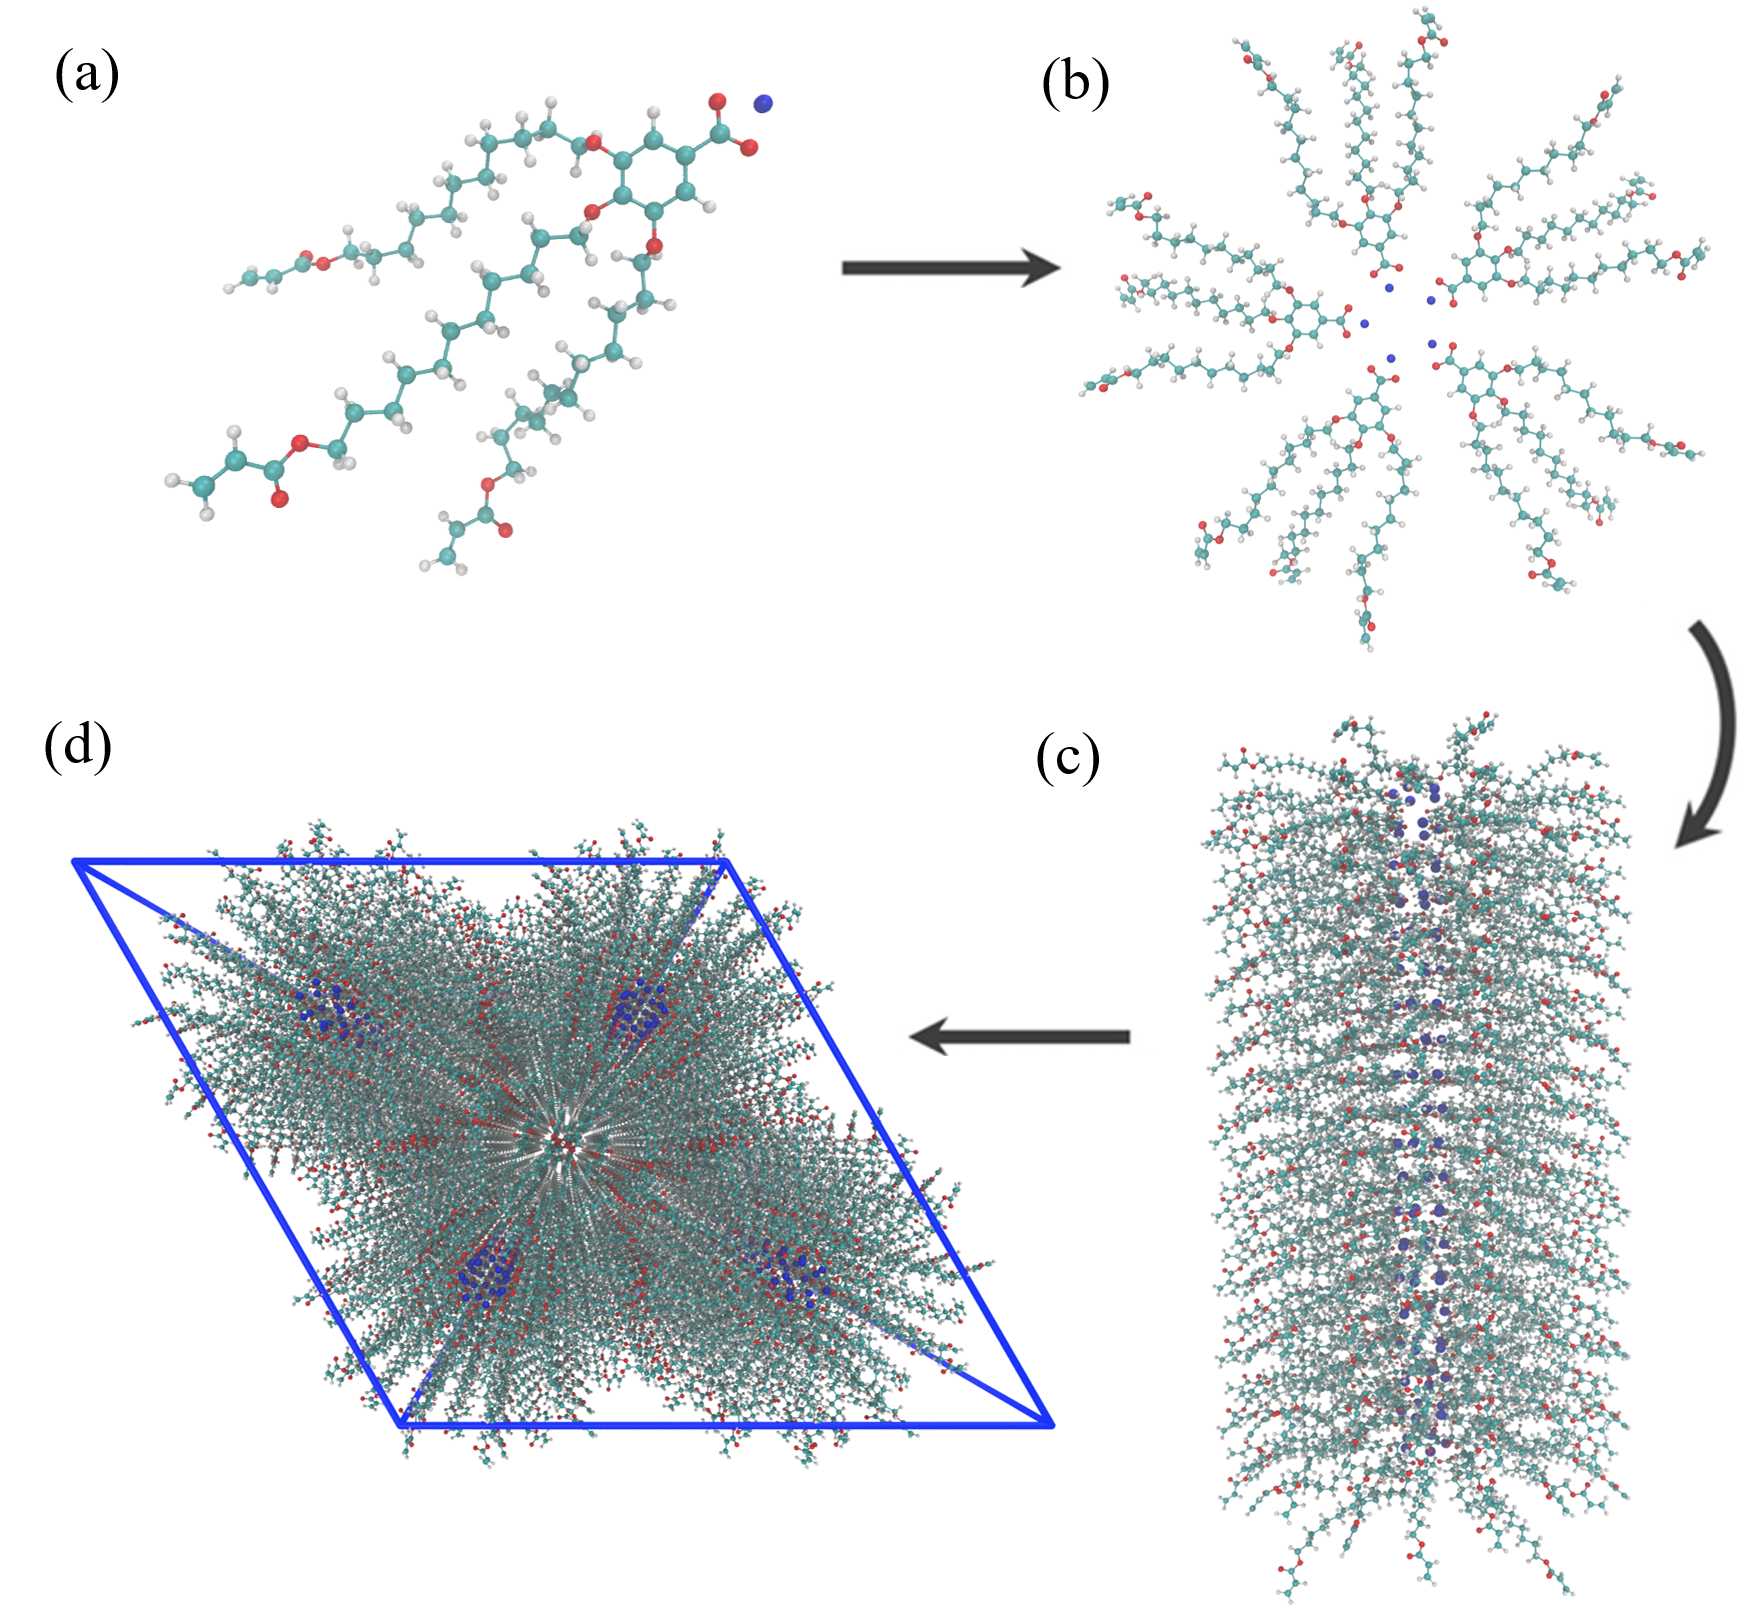
\includegraphics[width=0.75\linewidth]{build.PNG}
	\caption{(a) A single monomer was parameterized and annealed to produce a low energy
		configuration. (b) Monomers are rotated and assembled into layers with 
		hydrophlic centers. (c) Twenty layers are stacked on top of each other to create
		a pore. (d) Pores are duplicated and placed in a monoclinic unit cell}\label{fig:python}
\end{figure}

A typical simulation volume contains four pores in a monoclinic unit cell,
the smallest unit cell that maintains hexagonal symmetry when extended 
periodically. Each pore is made of twenty stacked monomer layers with
% describe unit cell in terms of alpha beta gamma angles?
% mention semi-isotropic pressure coupling here or later
periodic continuity in all directions, avoiding any edge effects and 
creating an infinite length pore ideal for studying transport. A small
number of layers is preferred in order to reduce computational cost and 
to allow us to look at longer timescales. Ultimately, we chose to build a 
system with 20 monomer layers in each pore in order to   
obtain sufficient resolution when simulating X-ray diffraction patterns.
This point will be explained in more detail later. 
% BJC: reword / mention xrd resolution - system size dependence in previous sentence

% Questionably needed figure
%\begin{figure}
%
\includegraphics{placeholder.png}
%	\caption{Monomers are placed in an initial configuration close to
%	         the expected equilibrium configuration and allowed to relax}
%	\label{fig:initial}
%\end{figure}

Initial guesses for the remaining structural parameters were chosen
based on experimental data and treated as variables during model
development. The distance between pores was based on experimental SAXS
data for this system \cite{feng_thin_2016}. Initial configuration pore
spacing was chosen to be 10 \% larger than the experimental value to reduce
unintended repulsions resulting from a tightly packed initial configuration. 
The layer spacing was based on experimental 2D WAXS data which shows
reflections corresponding to features spaced 3.7 \angstrom apart. It has 
been hypothesized that the features are present due to pi-pi
interactions between stacked aromatic rings \cite{feng_scalable_2014}. 
Our simulations tend to equilibrate to a wider interlayer spacing of $\approx$ 4.1 \angstrom,
which inspired separate systems starting with layer spacings greater than
 4 \angstrom. We estimate the pore radius to be 0.6 nm based on past TEM 
images and size exclusion rejection data\cite{feng_scalable_2014,
feng_thin_2016,zhou_supported_2005}. Comparing a geometric
measurement of pore size taken from an atomistic model, to a less
precise, experimentally derived pore size estimate, will give ambiguous
results. When constructing pores, we chose the carboxylate carbon from
the monomer head group as a reference atom, and placed it a distance r from the
pore center, where r is the pore radius. We will not make direct comparisons
of pore radius between our model and experiment to avoid the ambiguity. 
% There is plenty I can say about initial configuration. Starting layers
% too far apart, too close, tilted initial configurations etc.
The relative interlayer orientation was chosen based on clues from diffraction
data as well as the various known stacking modes of benzene and substituted 
benzene rings: sandwiched, parallel-displaced and T-shaped ~\cite{sinnokrot_estimates_2002}
(\Cref{fig:sandwiched,fig:pd,fig:tshaped}). The T-shaped 
configuration was ruled out based on the inconsistency of its $\approx$ 
5 \angstrom equilibrium stacking distance ~\cite{sinnokrot_estimates_2002}. The system's preference
towards the sandwiched vs. parallel displaced stacking modes was left
to be explored. Visualization of each configuration 
(\Cref{fig:sandwichedlayers,fig:offsetlayers}) suggests 
entropic differences based on the way the tails are able to pack.
In the sandwiched configuration, all tails start out directly on top 
of each other which may prevent closely stacked benzene rings. In the offset
configuration, the tails are placed in between each other which may allow layers
to come together in a compact way. This difference may explain, in part,
which stacking mode is more favorable.

\begin{figure}[ht]
	\centering
	\begin{subfigure}[b]{0.32\textwidth}
		\centering
		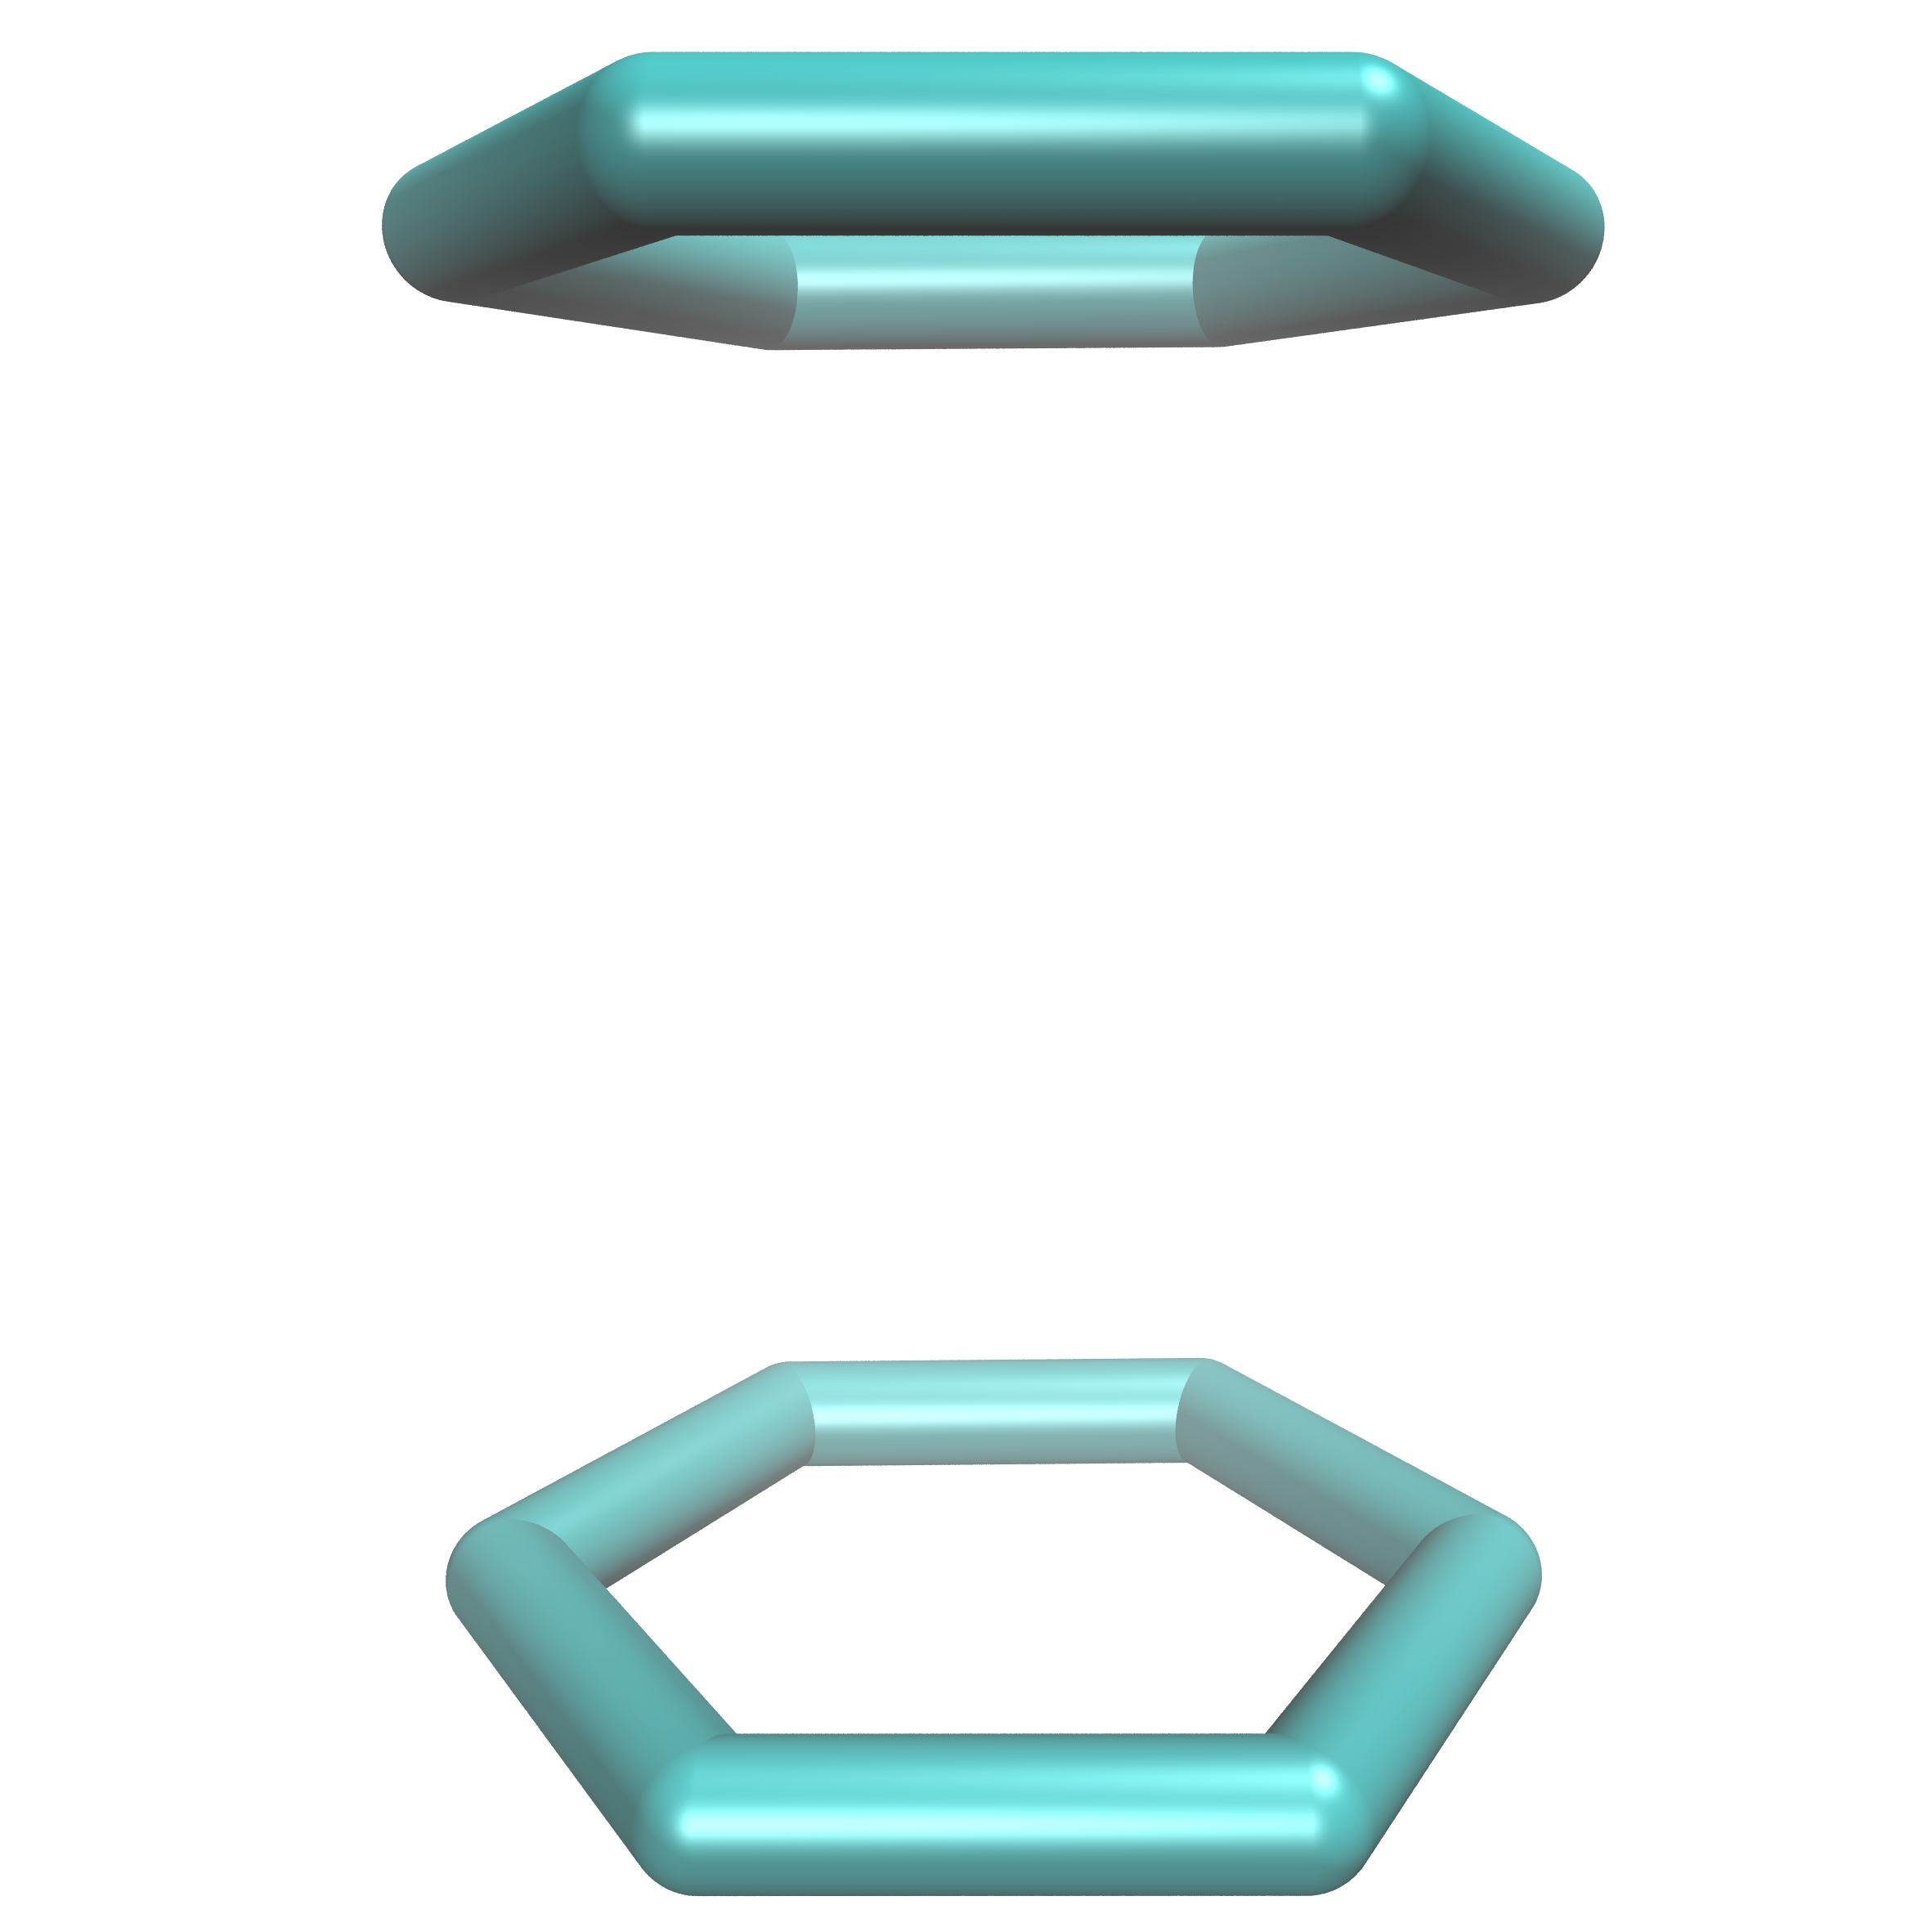
\includegraphics[width=\textwidth]{sandwiched.png}
		\caption{Sandwiched benzene dimers stack 3.8 \anstrom apart}\label{fig:sandwiched}
	\end{subfigure}
	\begin{subfigure}[b]{0.32\textwidth}
		\centering
		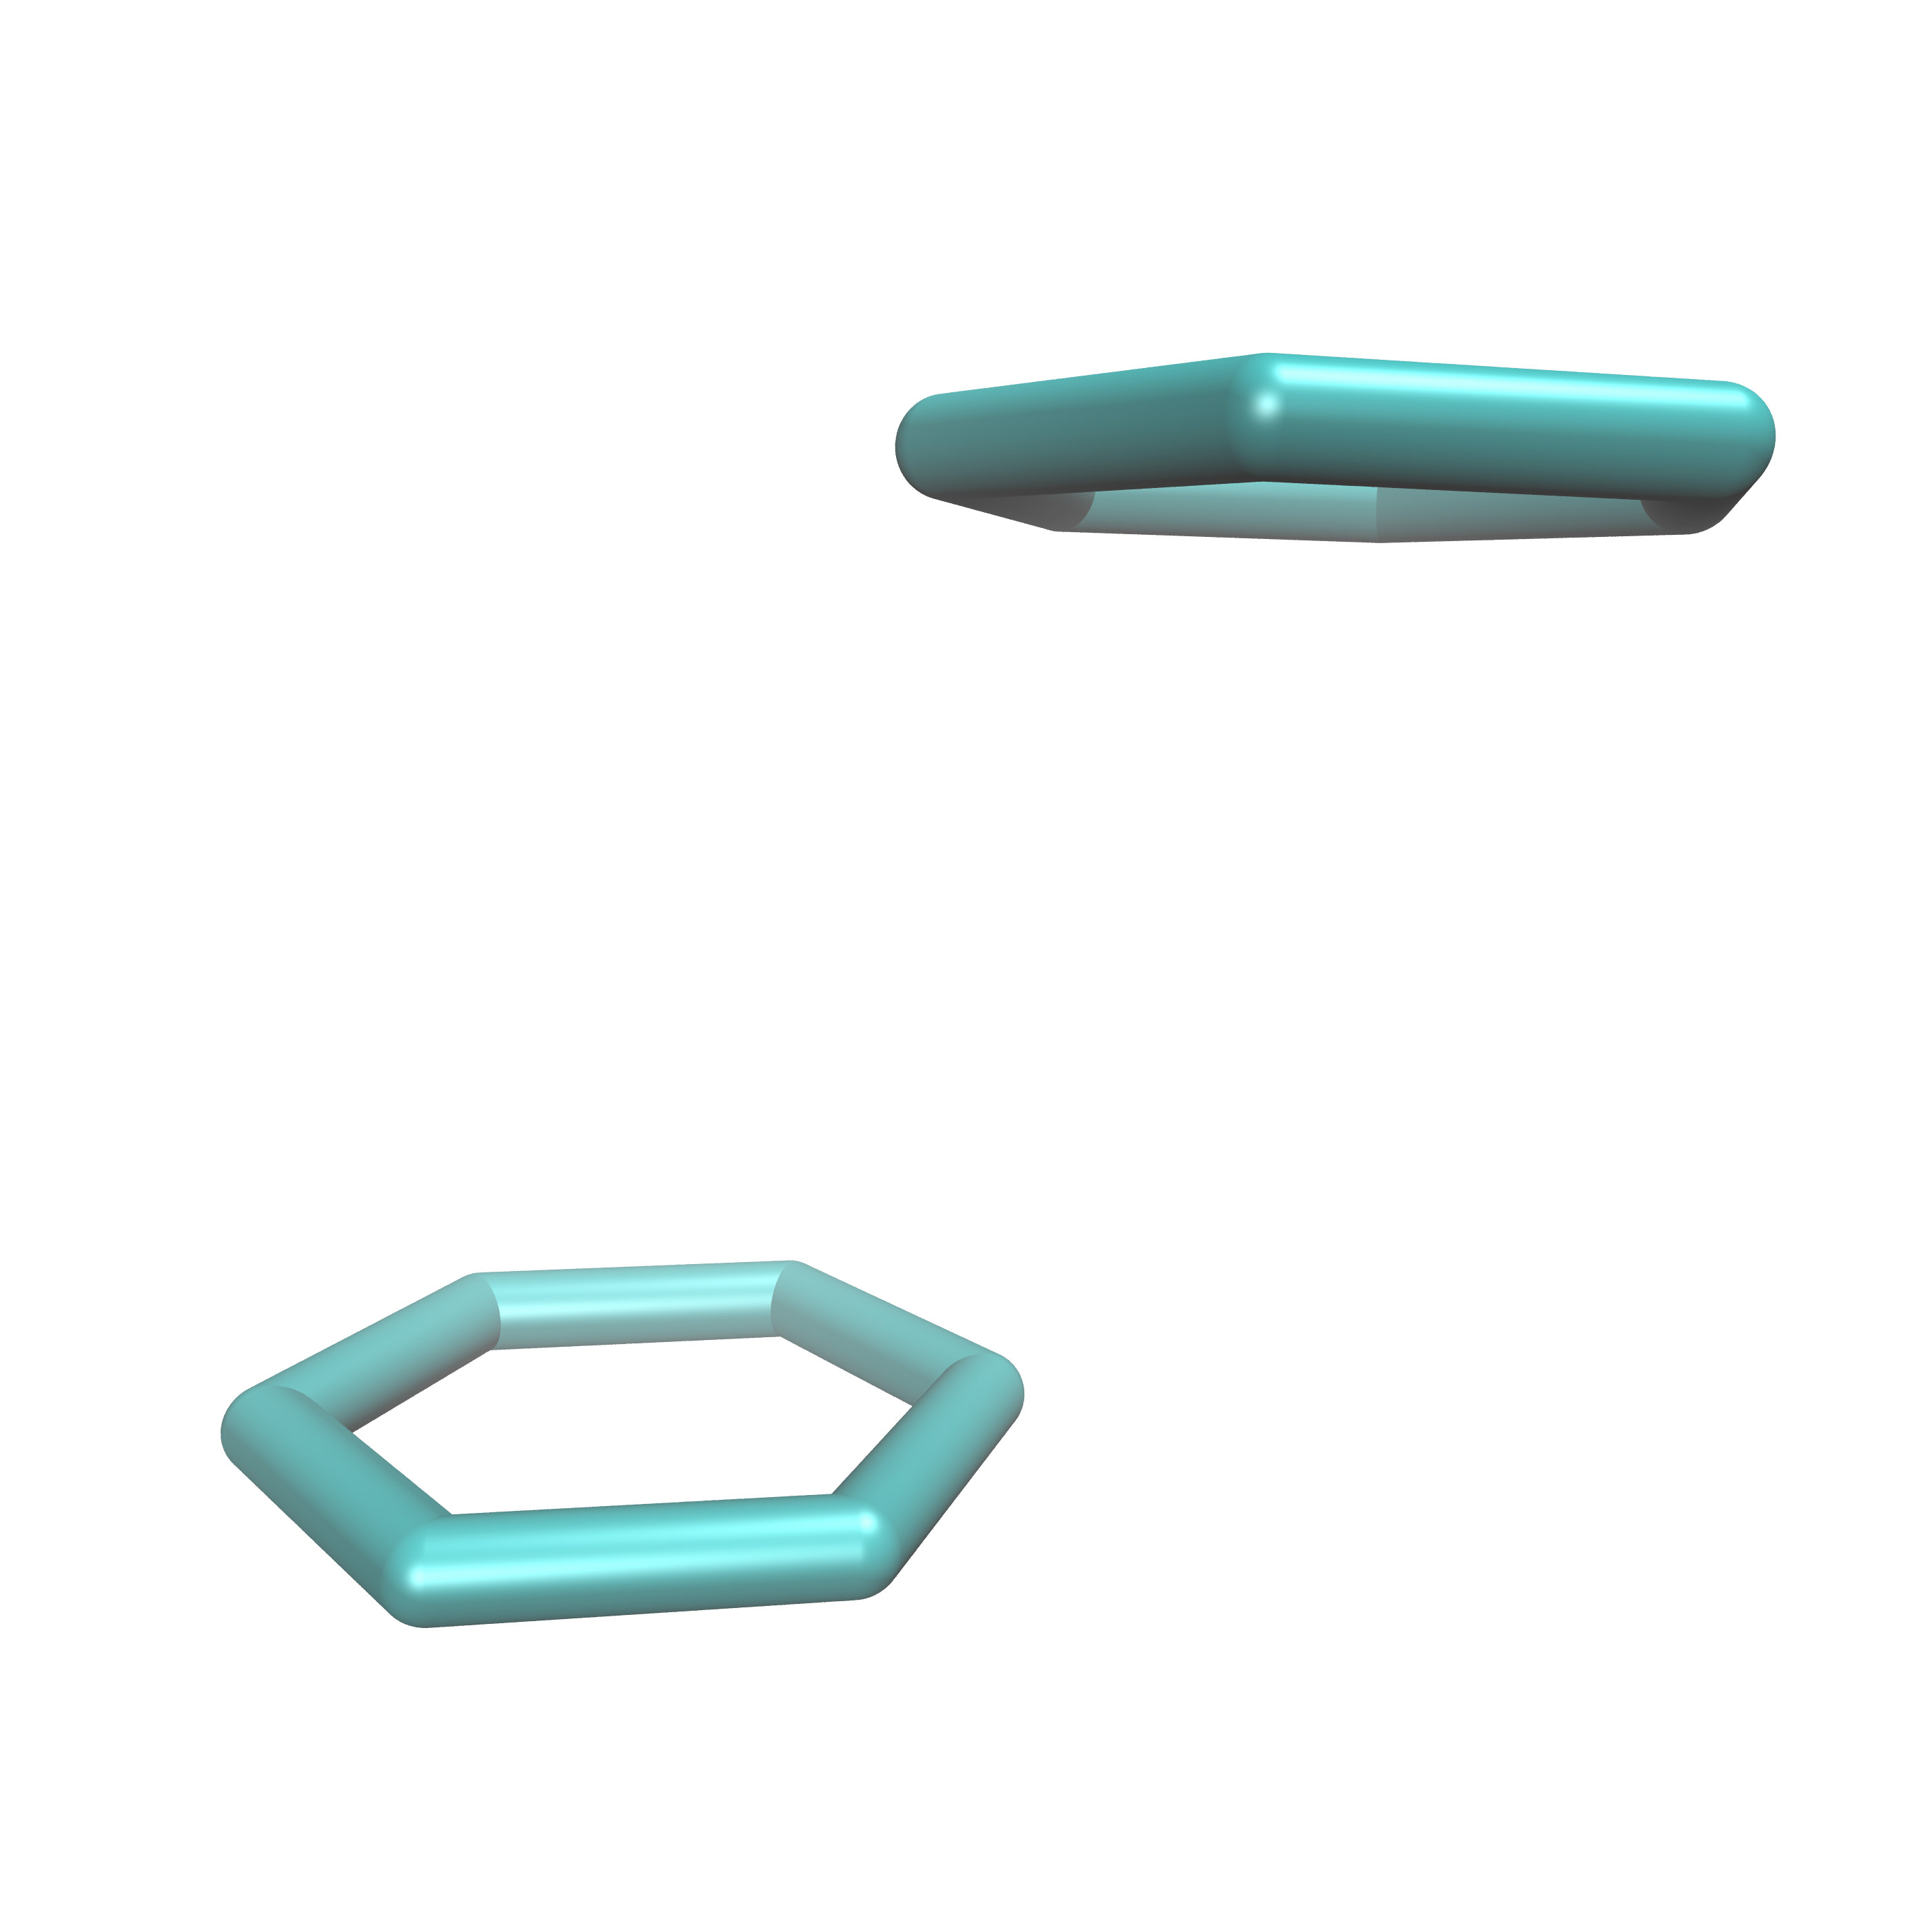
\includegraphics[width=\textwidth]{PD.png}
		\caption{Parallel-Displaced benzene dimers stack 3.4 \angstrom vertically and 1.6 \angstrom horizontally apart}\label{fig:pd}
	\end{subfigure}
	\begin{subfigure}[b]{0.32\textwidth}
		\centering
		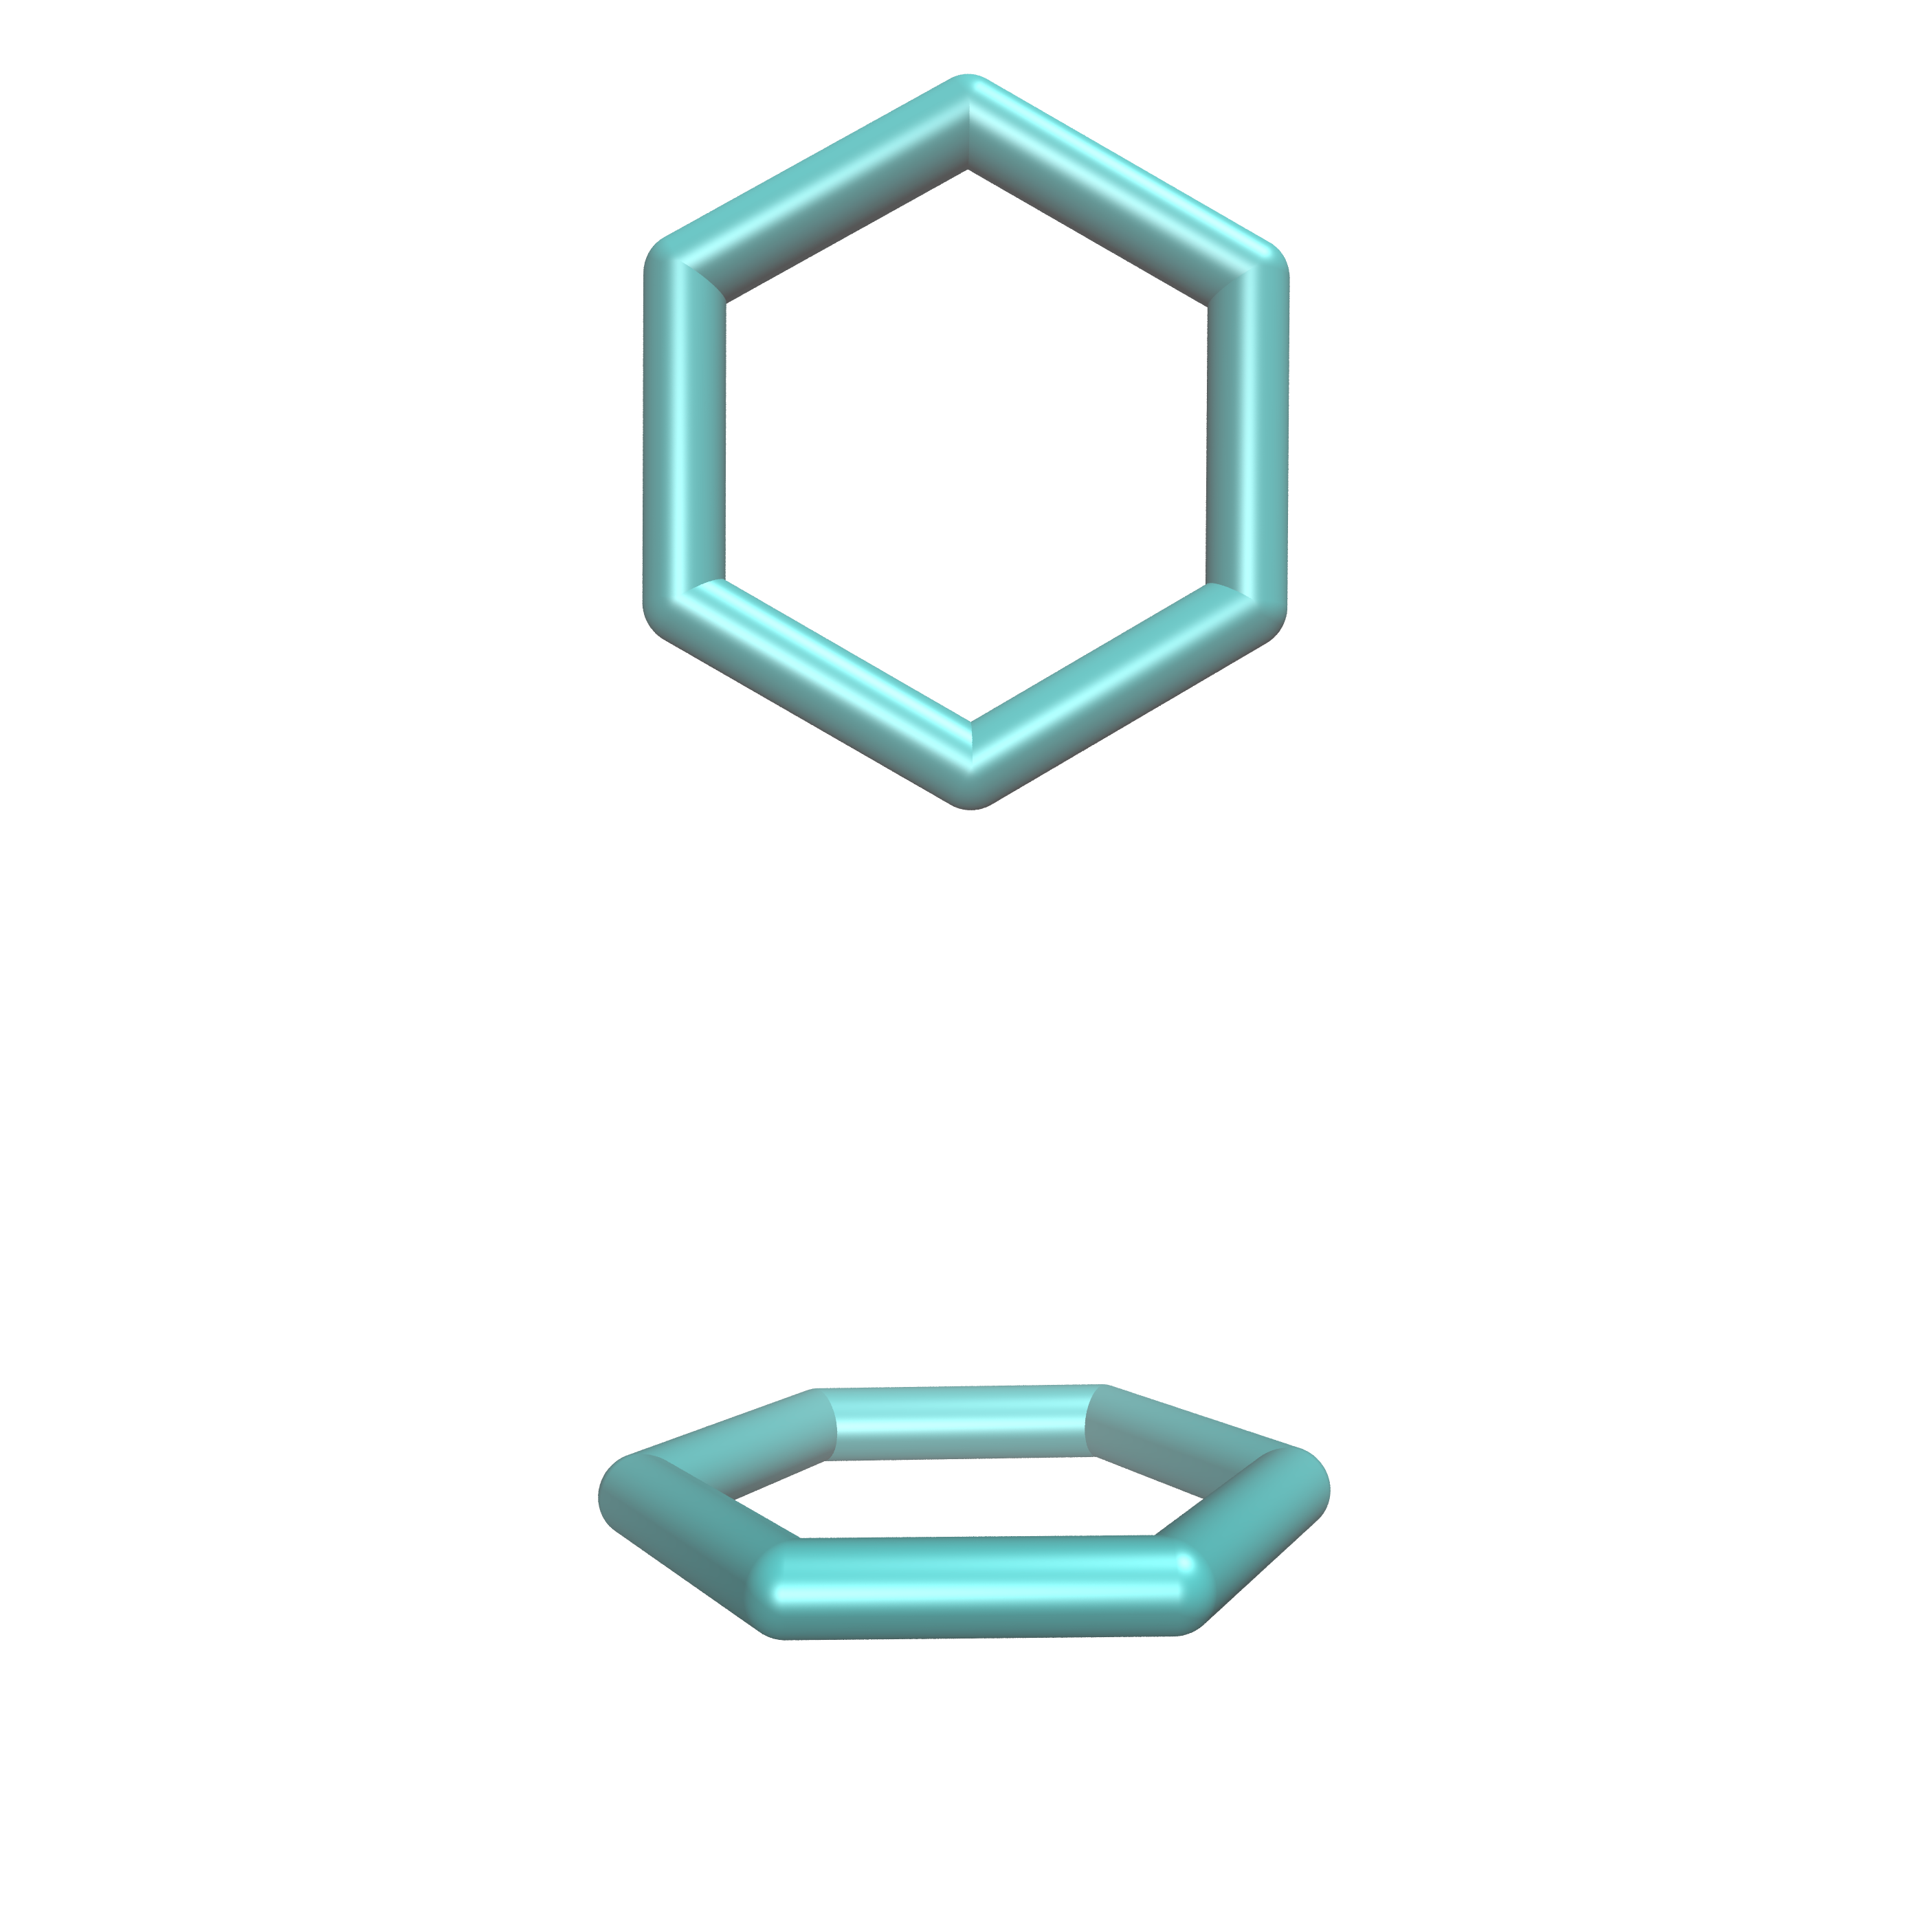
\includegraphics[width=\textwidth]{Tshaped.png}
		\caption{T-shaped benzene dimers stack 5.0 \angstrom apart}\label{fig:tshaped}
	\end{subfigure}
	\vskip\baselineskip
	\begin{subfigure}[b]{0.475\textwidth}
		\centering
		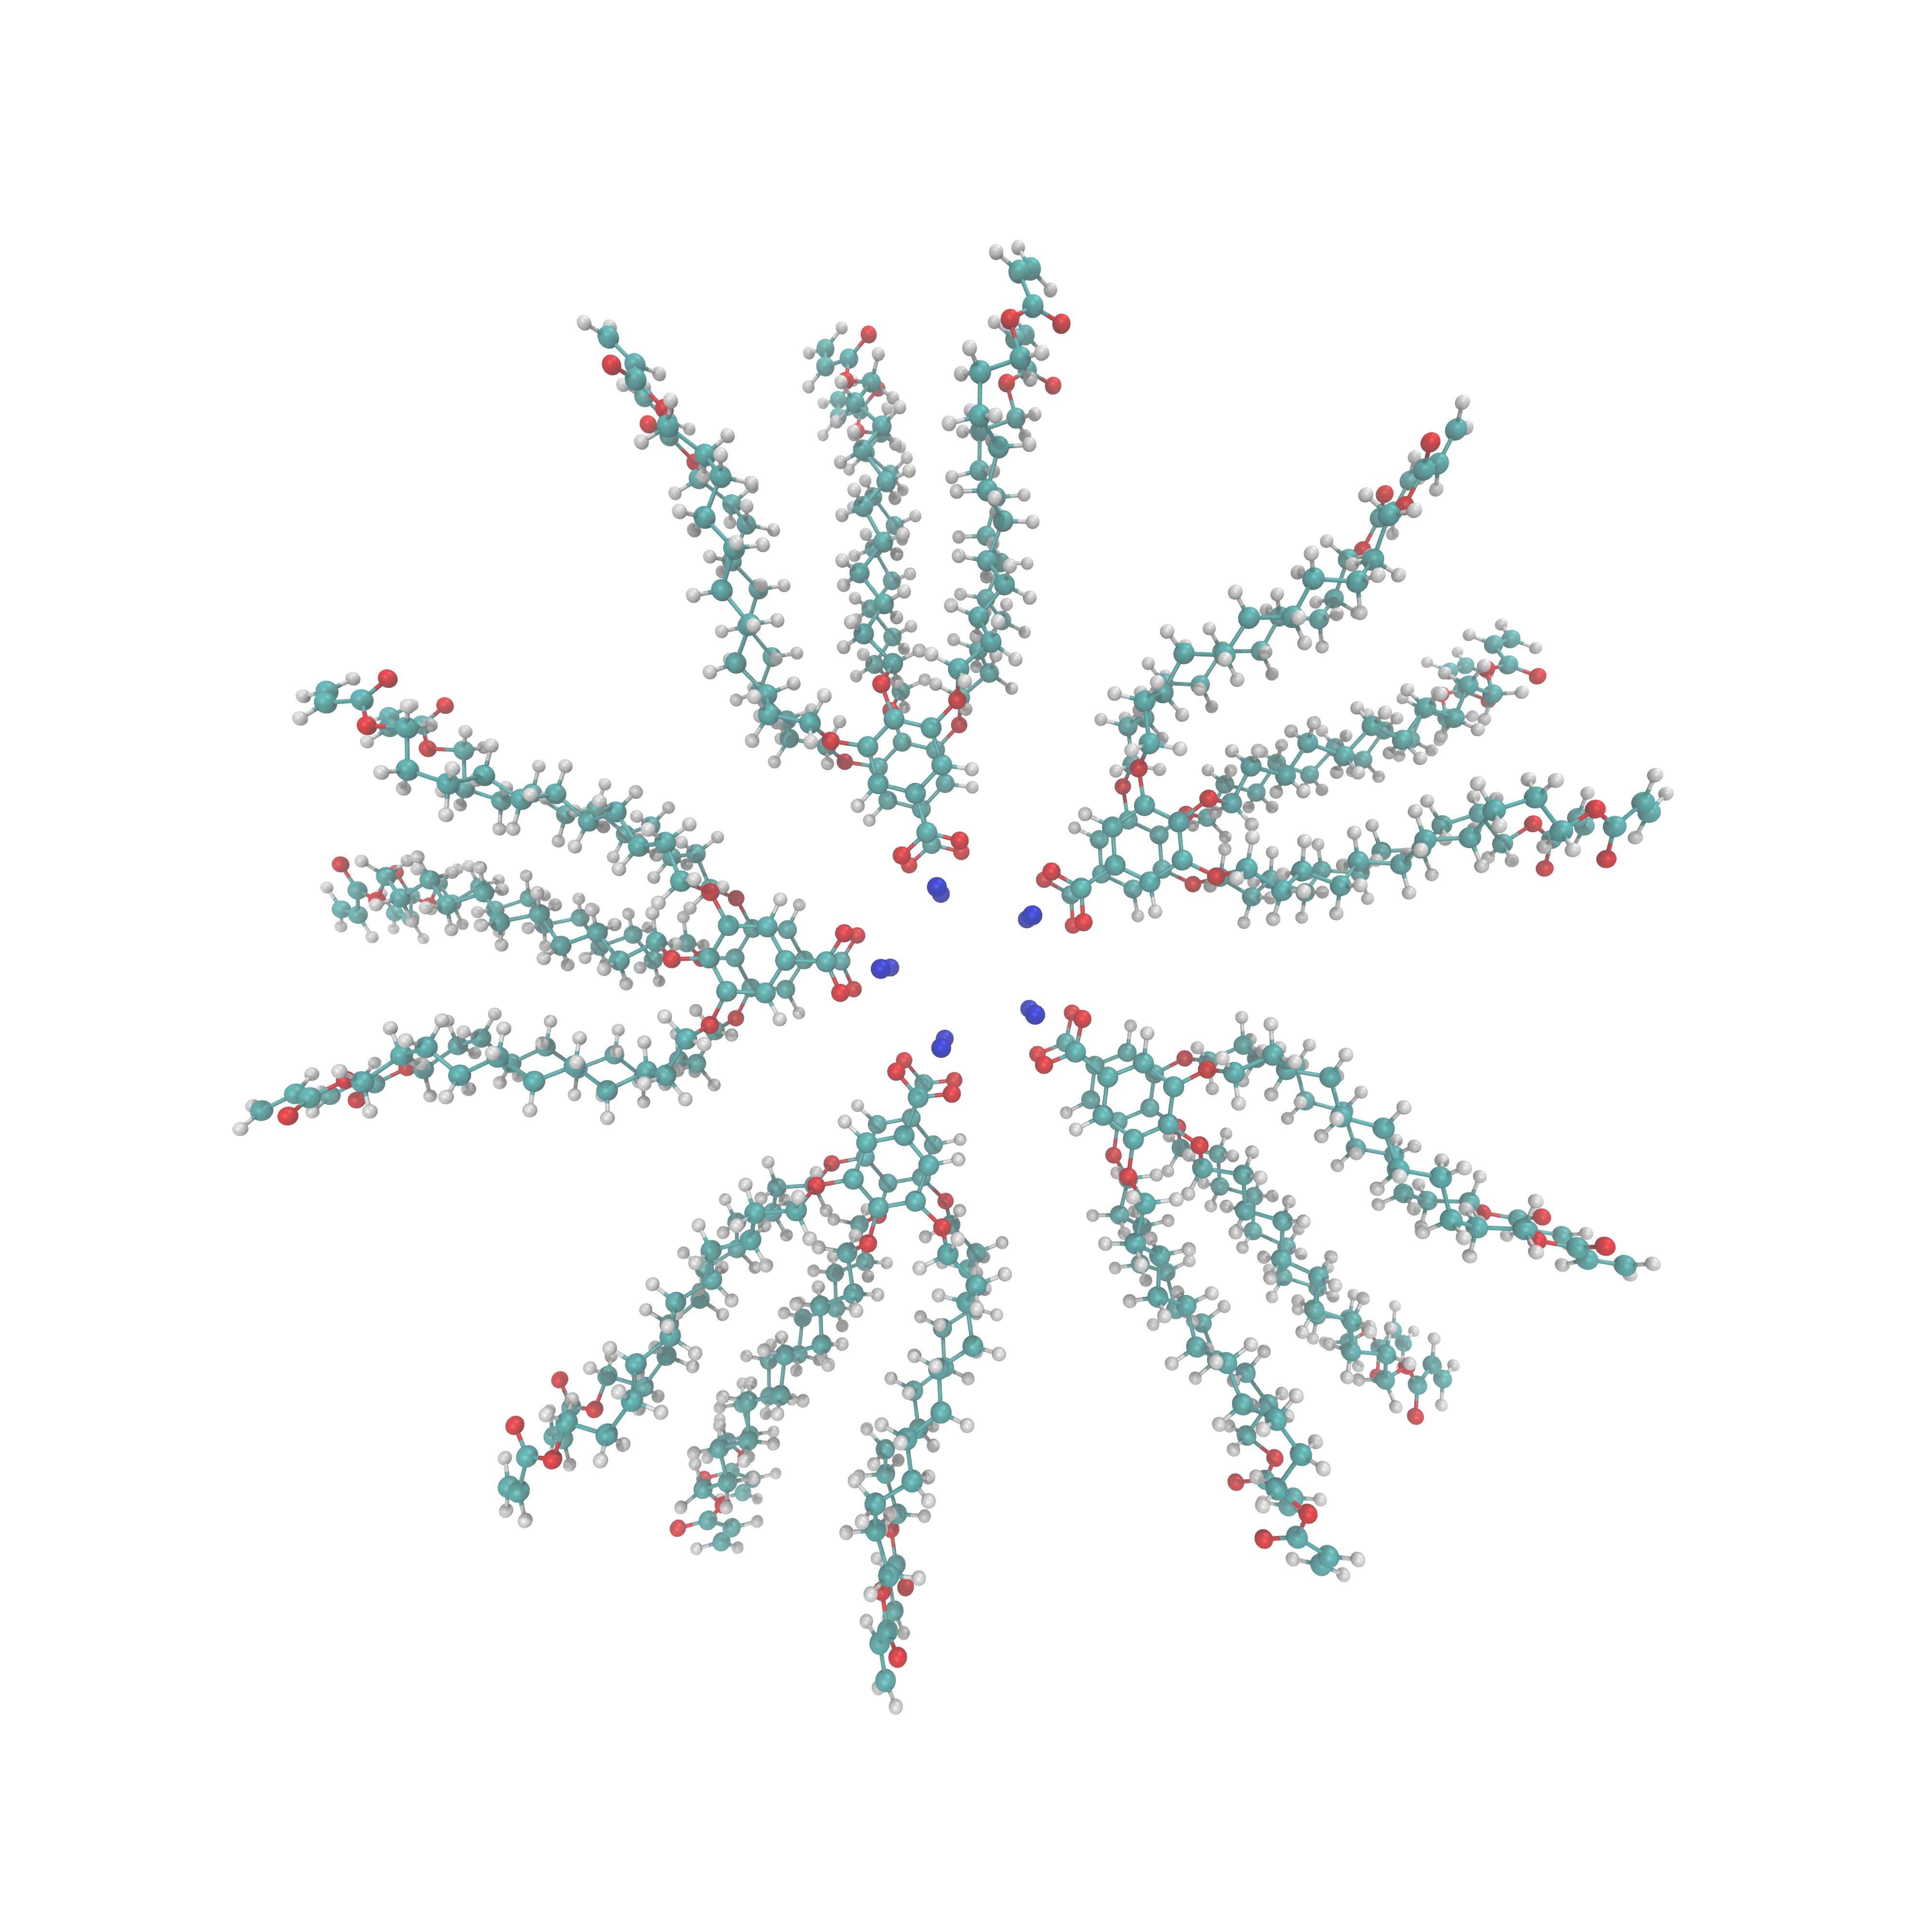
\includegraphics[width=\textwidth]{sandwichedlayers.png}
		\caption{Two monomer layers stacked in the sandwiched configuration}\label{fig:sandwichedlayers}
	\end{subfigure}
	\begin{subfigure}[b]{0.475\textwidth}
		\centering
		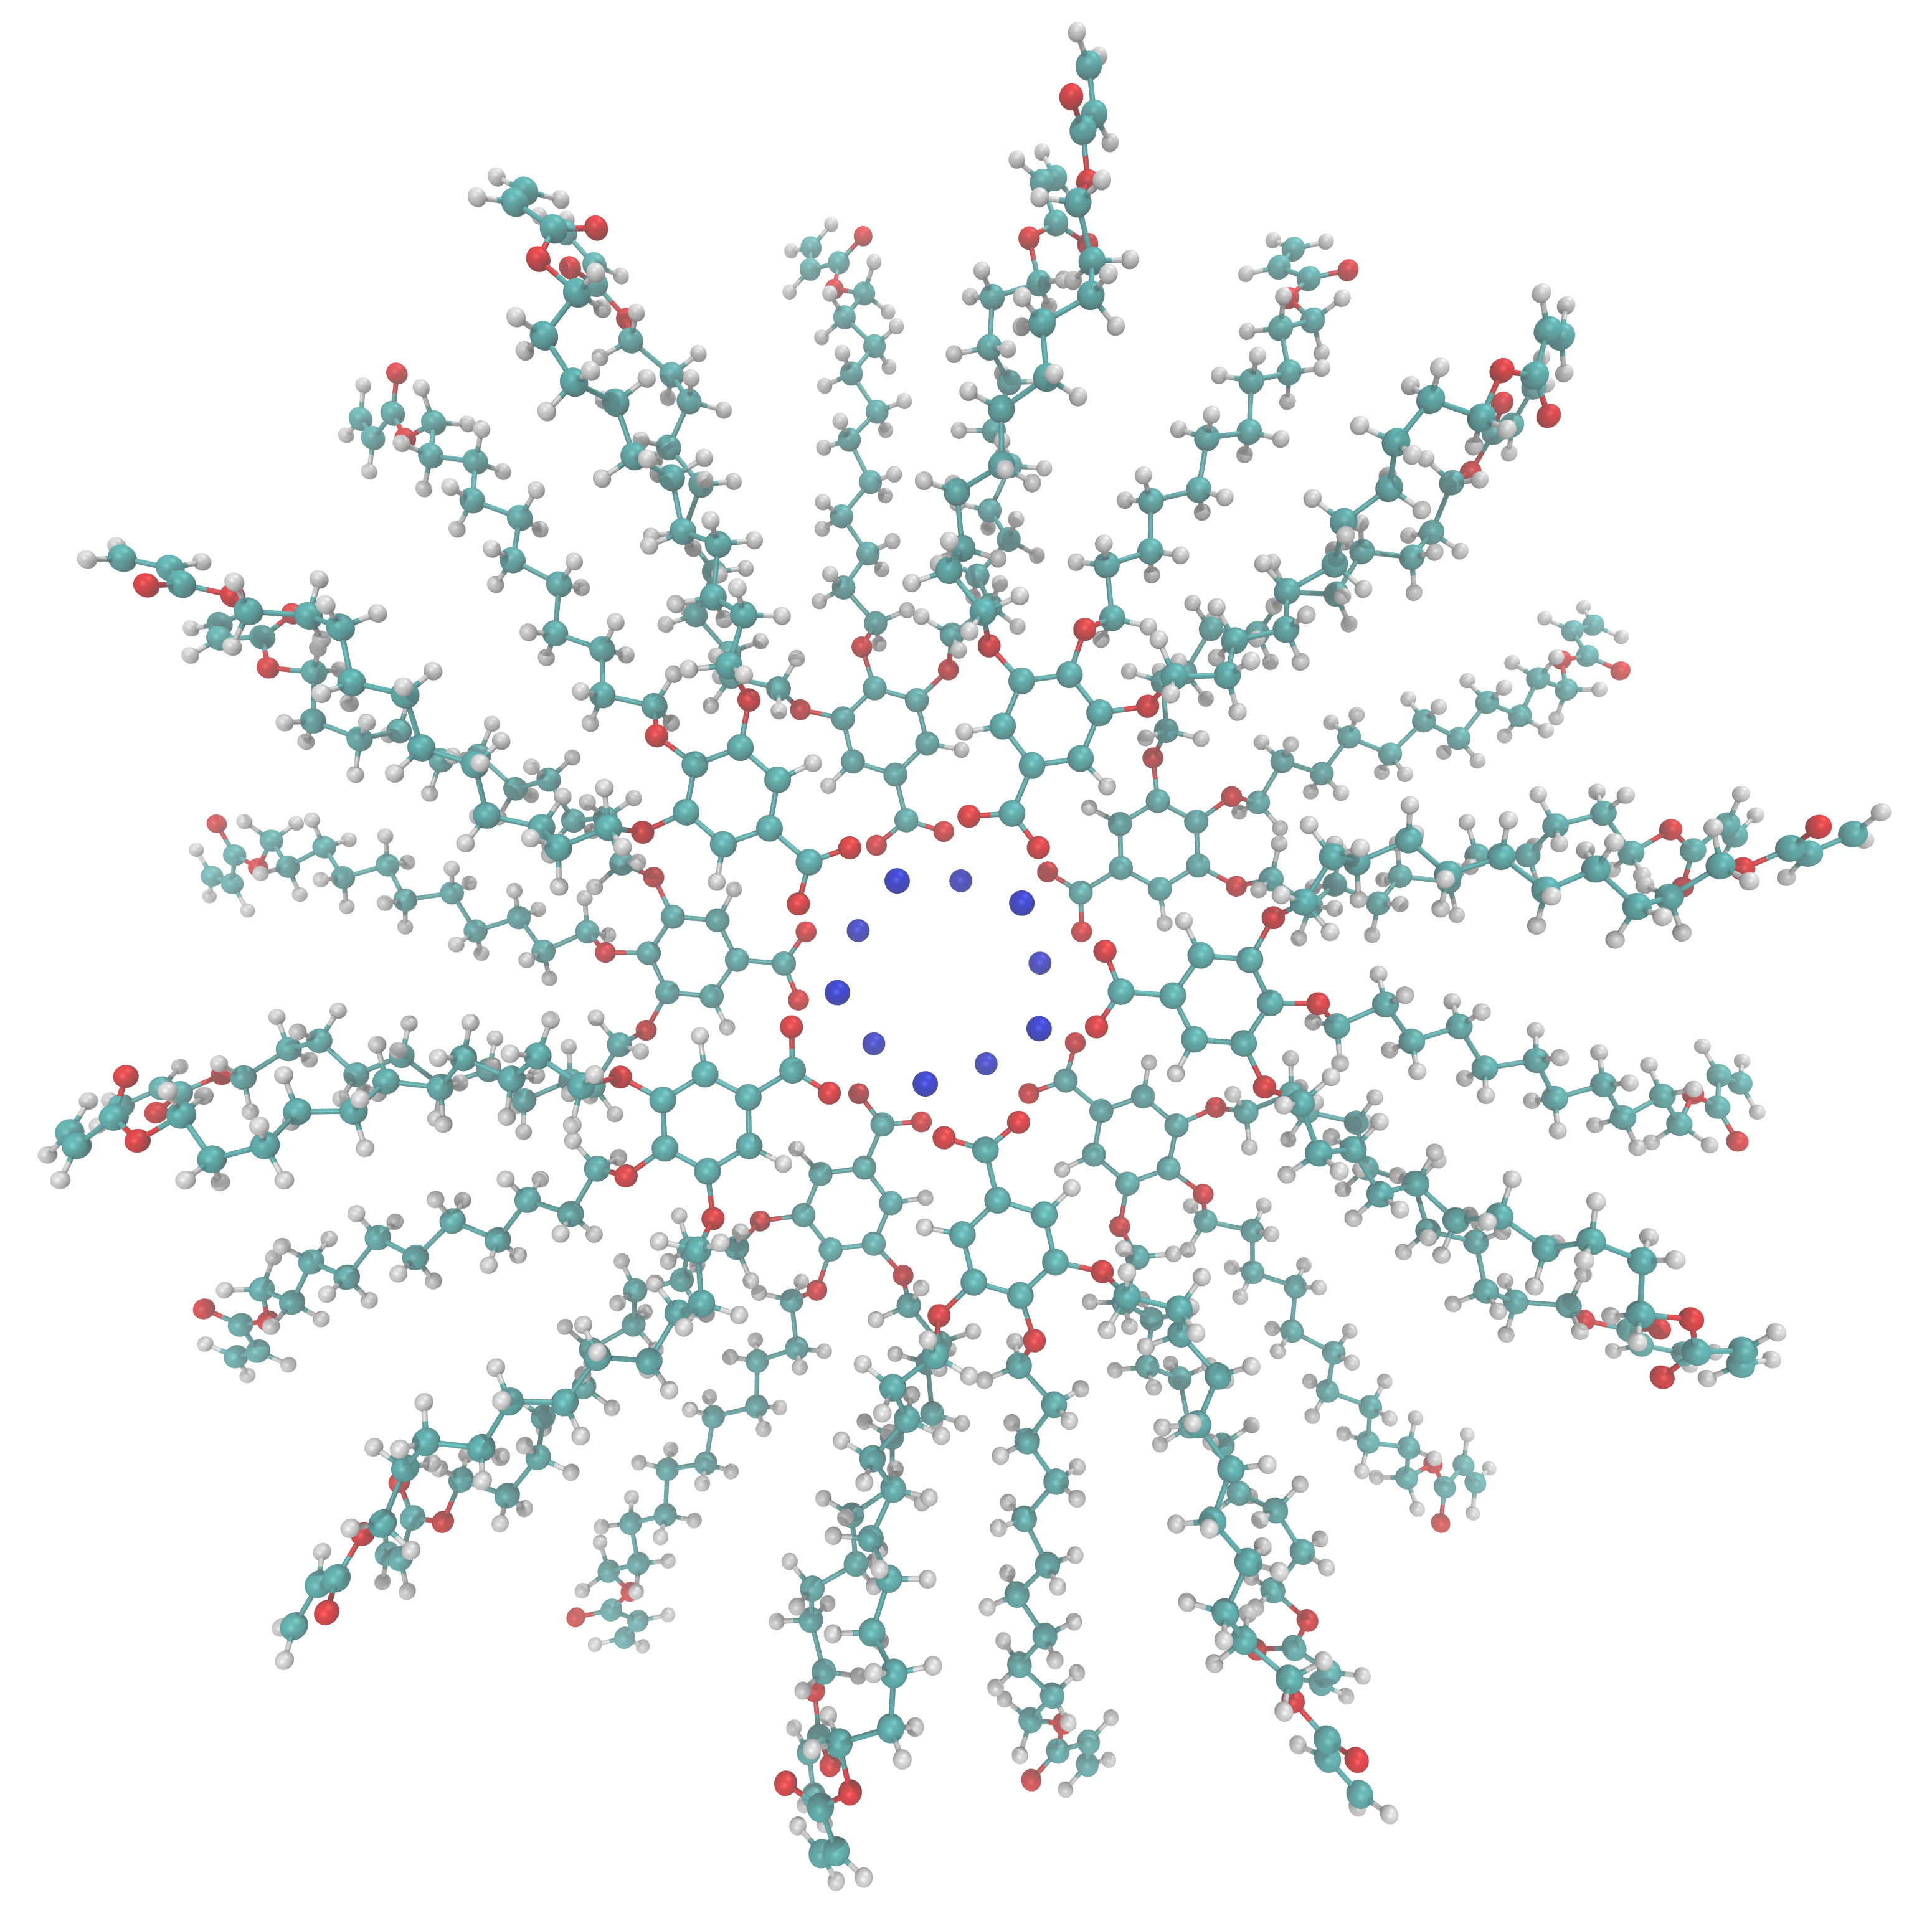
\includegraphics[width=\textwidth]{offsetlayers.png}
		\caption{Two monomer layers stacked in the parallel-displaced configuration}\label{fig:offsetlayers}
	\end{subfigure}
	\caption{}\label{fig:stacking}
\end{figure}

An equilibration scheme with position restraints placed on aromatic rings
prevents unrealistic jumps during early equilibration steps. Restraints
fix monomer head groups in the sandwiched or parallel-displaced 
configurations while allowing monomer tails to settle. Doing so also mitigates 
system dependence on initial monomer configuration. Restrained
equilibrations are run in the NVT ensemble. Every 50 ps, we reduce the force constants 
by the square root of its previous value, starting from 
1e6 KJ mol\textsuperscript{-1} nm\textsuperscript{-2}. Once the force constant
is below 10 KJ mol\textsuperscript{-1} nm\textsuperscript{-2}, the 
restraints are slowly released until there is no more restraining 
potential. The resulting unrestrained structure is allowed to 
equilibrate in the NPT ensemble for 400 - 500 ns. 

%Determination of equilibration 
%\begin{itemize}
%	\item Pore spacing 
%	\item Benzene ring stacking
%\end{itemize} 

Simulated X-ray diffraction patterns were generated based on atomic
coordinates for a direct experimental comparison. All atomic coordinates
were simulated as gaussian spheres of electron density corresponding to
each atom's atomic number. A three dimensional fourier transform 
(FT) of the array of electron density results in a three dimensional structure
factor whicih represents the unit cell in reciprocal space. We perform an
angular average of the structure factor about the z axis to generate a
2D cross section close to what one would see experimentally. We matched 
experimental 2D WAXS patterns by iterative improvement of our choice of 
initial structure and equilibration procedure. 
% Replace with a description written by Joe eventually

Ionic conductivity was calculated using two different methods for
robustness. The Nernst-Einstein relation relates 
the DC ionic conductivity to ion diffusivity, $D$, concentration,
$C$, ion charge, $q$, the boltzmann constant, $k_b$, and temperature,
$T$: $$\sigma = \dfrac{q^2CD}{k_b T}$$ Sodium ion diffusion 
coefficients were found by calculating the slope of the linear
region of the mean square displacement curve as indicated by the
einstein relation \cite{einstein_investigations_1956}. Ion concentration
was measured with respect to the entire unit cell. The second method, 
termed the 'Collective Diffusion' model \cite{liu_collective_2013}, 
measures the movement of the collective variable, Q, which is defined as
the amount of charge transfer through the system. The diffusion 
coefficient of Q, $D_Q$, can be calculated using the einstein relation.
The conductance, $\gamma$ of the system can be calculated as:
$$ \gamma = \dfrac{D_Q}{k_b T} $$ Conversion to ionic conductivity is
achieved by multiplying by channel length and dividing by the membrane
cross sectional area. A full derivation of the model can be accessed 
elsewhere \cite{liu_collective_2013}.  
% Talk about error somewhere?

Using an equilibrated structure, a crosslinking procedure was performed
in order to better parallel synthetic procedures. The purpose of 
crosslinking is to maintain macroscopic alignment of the crystalline
domains, ensuring aligned, hexagonally packed pores. For that reason, we
are not concerned with replicating the kinetics of the reaction, but
instead emphasize the consistency of the final structure with experimental
structural data. The algorithm was developed based on the known reaction
mechanism. Crosslinking of this system is a free radical polymerization (FRP)
taking place between terminal vinyl groups present on each of the three
monomer tails. FRPs require an initiator which bonds to the system, 
meaning new atoms were introduced into the system. For simplicity, the 
initiator was simulated as hydrogen and made present in the simulation
by including them in all possible bonding positions as dummy atoms.
The crosslinking procedure is carried out iteratively. During each 
iteration, bonding carbon atoms are chosen based on a distance cut-off.
The topology is updated with new bonds and dummy hydrogen atoms are 
changed to appropriate hydrogen types. Head-to-tail addition was the
only propagation mode considered due to its dominance in real systems.
Direction of attack was not considered because the resultant mixture is
racemic. The resulting crosslinked structure has an even distribution of
crosslinks between monomer tails of the same monomer, monomers stacked on
top of each other and monomers in other pores, including across periodic
boundaries. The pore spacing shrinks by $\approx$ 1 \angstrom and stays 
constant under a range of simulation conditions. 
